\begin{Problem}
	Betrachten Sie die folgenden Familien von Kraftfeldern auf geeigneten Definitionsbereichen $D_\eta^{(n)}  \subseteq \R^3$
	\begin{align*}
		F_\eta^{(1)}:& D_\eta^{(1)}\ni \va x\to r^\eta\cdot \va x\in \R^3\\
		F_\eta^{(2)}:& D_\eta^{(2)}\ni\va x \to r_{12}^\eta\cdot(x_1\va e_1-x_2\va e_2)\in \R^3\\
		F_\eta^{(3)}:& D_\eta^{(3)}\ni \va x\to r_{12}^\eta\cdot\left( x_2\va e_1-x_1\va e_2 \right) \in\R^3\\
		F_\eta^{(4)}:&D_\eta^{(3)}\ni \va x\to r_{12}^\eta\cdot\left( x_2\va e_1+x_1\va e_2 \right) \in \R^3
	\end{align*}
	wobei $r_{12}=\sqrt{x_1^2+x_2^2} $ und $r=\sqrt{x_1^2+x_2^2+x_3^3} $
	Skizzieren Sie die Felder $\va F_\eta^{(n)}$ als Vektorpfeile in der von den Einheitsvektoren $\va e_1$ und $\va e_2$ aufgespannten Ebene (hier genügt es, zwischen den Fällen $\eta > -1, \eta = -1$ und $\eta < -1$ zu unterscheiden). 
	
	Bestimmen Sie, abhängig von der Potenz $\eta \in \R$,
	\begin{enumerate}
		\item den maximalen Definitionsbereich $D_\eta^{(n)}$,
		\item die maximale Bereiche $C_\eta^{(n)}\subseteq D_\eta^{(n)}$, auf denen $F_\eta^{(n)}$ konservativ ist,
		\item eine Potentialfunktion $V_\eta^{(n)}:C_{\eta}^{(n)}\to \R$ mit $F_\eta^{(n)}=-\grad{V_\eta^{(n)}}$, sofern sie existiert,
		\item das Kurvenintegral
		\[I_\eta^{(n)}(R)=\int_{\gamma_R}\dd{\va\xi}\cdot\va F_\eta^{(n)}(\va\xi)\]
		über den gegen den Uhrzeigersinn umlaufenen Kreis $\gamma_R$ mit Radius $R$ und Mittelpunkt $\va0$ in der von $\va e_1$ und $\va e_2$ aufgespannten Ebene
		\begin{center}
			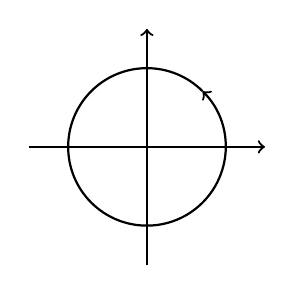
\begin{tikzpicture}
				\draw[thick, ->] (-1.5,0) -- (1.5,0);
				\draw[thick, ->] (0,-1.5) -- (0,1.5);
				\draw[thick, ->] ({1/sqrt(2)},{1/sqrt(2)}) arc (45:405:1);
			\end{tikzpicture}
		\end{center}
	\end{enumerate}
\end{Problem}


\begin{proof}
	\begin{figure}[h!]
		\begin{subcaptionbox}{$\eta>-1$}
	 {\resizebox{0.3\textwidth}{!}{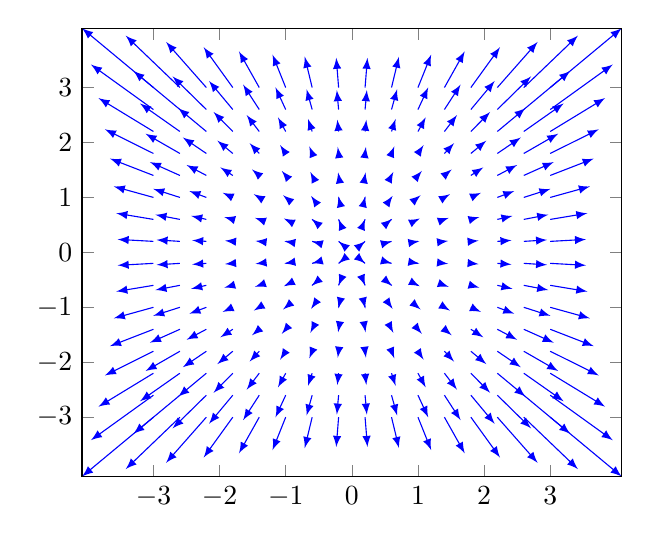
\begin{tikzpicture}
 \begin{axis}[%
  view     = {0}{90}, % for a view 'from above'
  domain   = -3:3,
  y domain = -3:3,
  xtick    = {-3,...,3},
  ytick    = {-3,...,3},
]
\addplot3[blue, quiver={u=(x*x+y*y)*x, v=(x*x+y*y)*y, scale arrows=0.02}, samples=16, -latex] (x,y,0);
\end{axis}
\end{tikzpicture}}}
	\begin{subcaptionbox}{$\eta=-1$}
	{\resizebox{0.3\textwidth}{!}{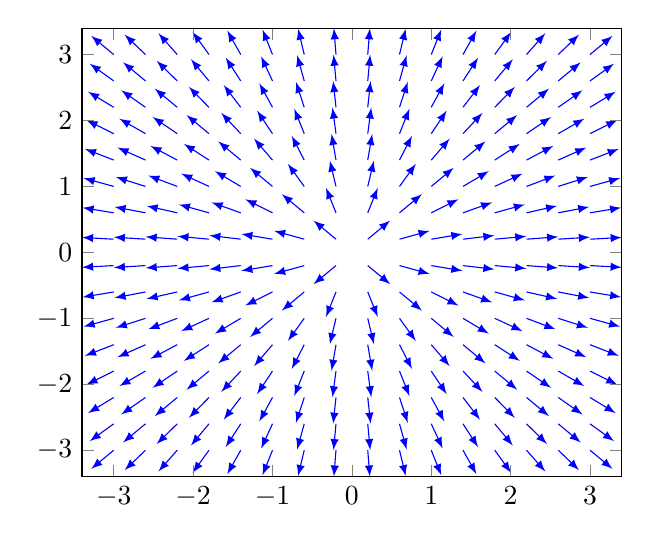
\begin{tikzpicture}
			\begin{axis}[%
				view     = {0}{90}, % for a view 'from above'
				domain   = -3:3,
				y domain = -3:3,
				xtick    = {-3,...,3},
				ytick    = {-3,...,3},
				]
				\addplot3[blue, quiver={u=x/(x*x+y*y)^(1/2), v=y/(x*x+y*y)^(1/2), scale arrows=0.4}, samples=16, -latex] (x,y,0);
			\end{axis}
	\end{tikzpicture}}}
\end{subcaptionbox}
\end{subcaptionbox}
	\begin{subcaptionbox}{$\eta<-1$}
	{\resizebox{0.3\textwidth}{!}{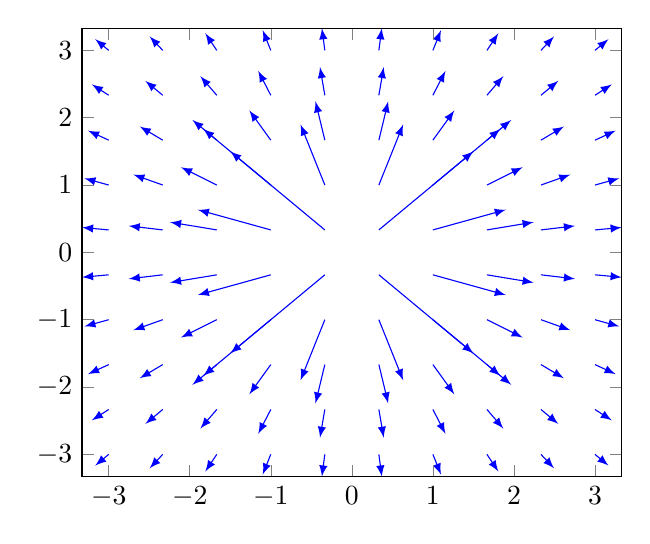
\begin{tikzpicture}
			\begin{axis}[%
				view     = {0}{90}, % for a view 'from above'
				domain   = -3:3,
				y domain = -3:3,
				xtick    = {-3,...,3},
				ytick    = {-3,...,3},
				]
				\addplot3[blue, quiver={u=x/(x*x+y*y), v=y/(x*x+y*y), scale arrows=1}, samples=10, -latex] (x,y,0);
			\end{axis}
	\end{tikzpicture}}}
\end{subcaptionbox}
\caption{Vektorpfeile f\"{u}r $\va F_\eta^{(1)}$}
\end{figure}
	\begin{figure}[h!]
	\begin{subcaptionbox}{$\eta>-1$}
		{\resizebox{0.3\textwidth}{!}{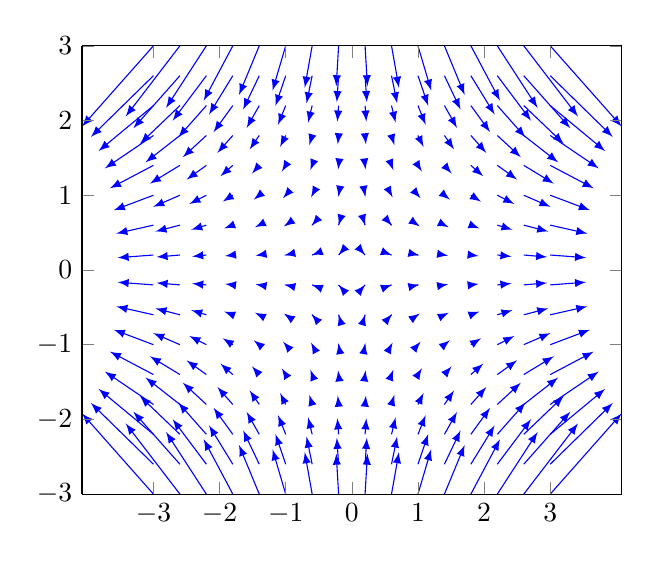
\begin{tikzpicture}
				\begin{axis}[%
					view     = {0}{90}, % for a view 'from above'
					domain   = -3:3,
					y domain = -3:3,
					xtick    = {-3,...,3},
					ytick    = {-3,...,3},
					]
					\addplot3[blue, quiver={u=(x*x+y*y)*x, v=-(x*x+y*y)*y, scale arrows=0.02}, samples=16, -latex] (x,y,0);
				\end{axis}
		\end{tikzpicture}}}
		\begin{subcaptionbox}{$\eta=-1$}
			{\resizebox{0.3\textwidth}{!}{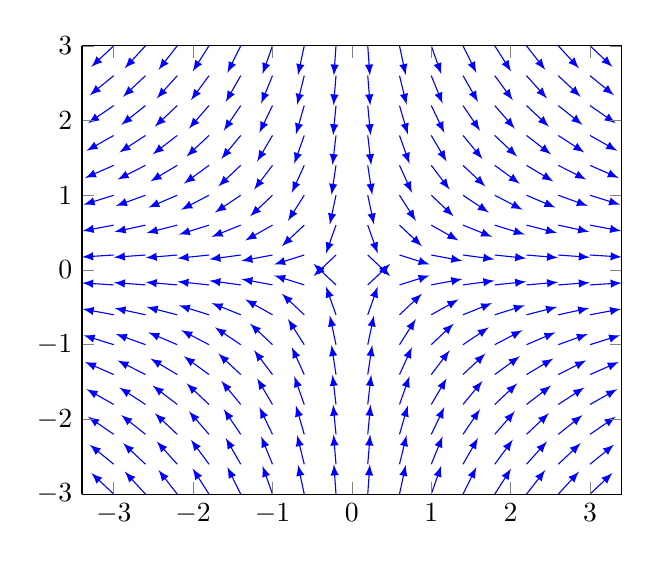
\begin{tikzpicture}
					\begin{axis}[%
						view     = {0}{90}, % for a view 'from above'
						domain   = -3:3,
						y domain = -3:3,
						xtick    = {-3,...,3},
						ytick    = {-3,...,3},
						]
						\addplot3[blue, quiver={u=x/(x*x+y*y)^(1/2), v=-y/(x*x+y*y)^(1/2), scale arrows=0.4}, samples=16, -latex] (x,y,0);
					\end{axis}
			\end{tikzpicture}}}
		\end{subcaptionbox}
	\end{subcaptionbox}
	\begin{subcaptionbox}{$\eta<-1$}
		{\resizebox{0.3\textwidth}{!}{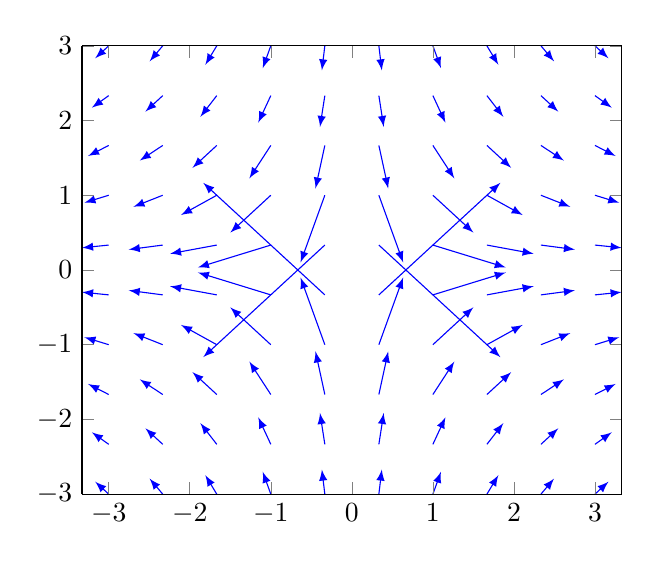
\begin{tikzpicture}
				\begin{axis}[%
					view     = {0}{90}, % for a view 'from above'
					domain   = -3:3,
					y domain = -3:3,
					xtick    = {-3,...,3},
					ytick    = {-3,...,3},
					]
					\addplot3[blue, quiver={u=x/(x*x+y*y), v=-y/(x*x+y*y), scale arrows=1}, samples=10, -latex] (x,y,0);
				\end{axis}
		\end{tikzpicture}}}
	\end{subcaptionbox}
	\caption{Vektorpfeile f\"{u}r $\va F_\eta^{(2)}$}
\end{figure}
	\begin{figure}[h!]
	\begin{subcaptionbox}{$\eta>-1$}
		{\resizebox{0.3\textwidth}{!}{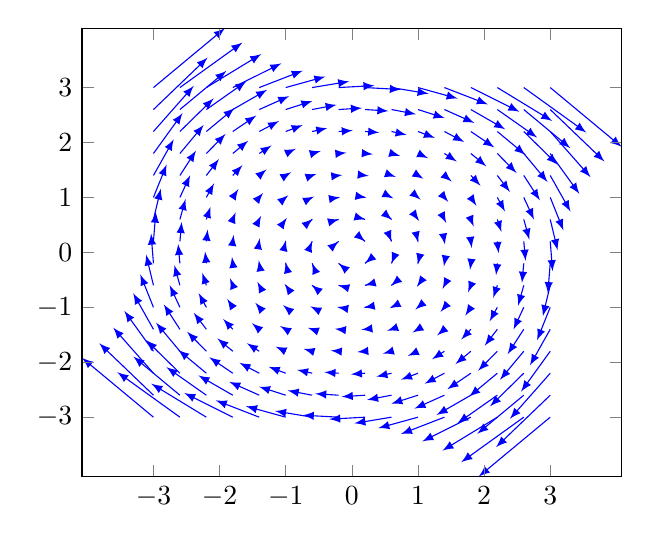
\begin{tikzpicture}
				\begin{axis}[%
					view     = {0}{90}, % for a view 'from above'
					domain   = -3:3,
					y domain = -3:3,
					xtick    = {-3,...,3},
					ytick    = {-3,...,3},
					]
					\addplot3[blue, quiver={u=(x*x+y*y)*y, v=-(x*x+y*y)*x, scale arrows=0.02}, samples=16, -latex] (x,y,0);
				\end{axis}
		\end{tikzpicture}}}
		\begin{subcaptionbox}{$\eta=-1$}
			{\resizebox{0.3\textwidth}{!}{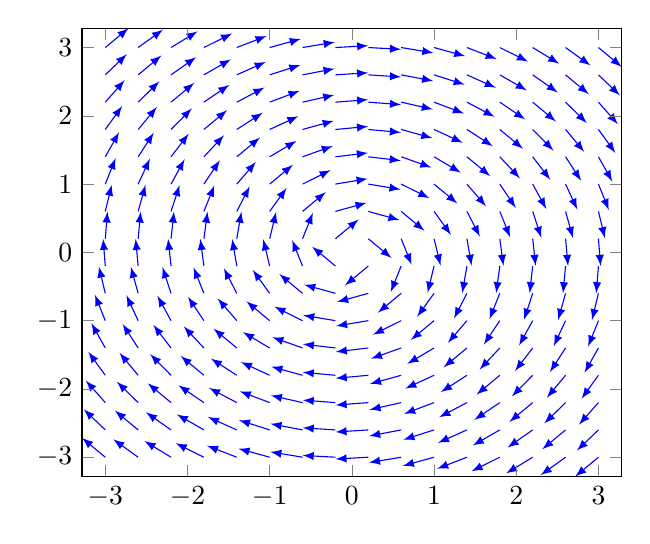
\begin{tikzpicture}
					\begin{axis}[%
						view     = {0}{90}, % for a view 'from above'
						domain   = -3:3,
						y domain = -3:3,
						xtick    = {-3,...,3},
						ytick    = {-3,...,3},
						]
						\addplot3[blue, quiver={u=y/(x*x+y*y)^(1/2), v=-x/(x*x+y*y)^(1/2), scale arrows=0.4}, samples=16, -latex] (x,y,0);
					\end{axis}
			\end{tikzpicture}}}
		\end{subcaptionbox}
	\end{subcaptionbox}
	\begin{subcaptionbox}{$\eta<-1$}
		{\resizebox{0.3\textwidth}{!}{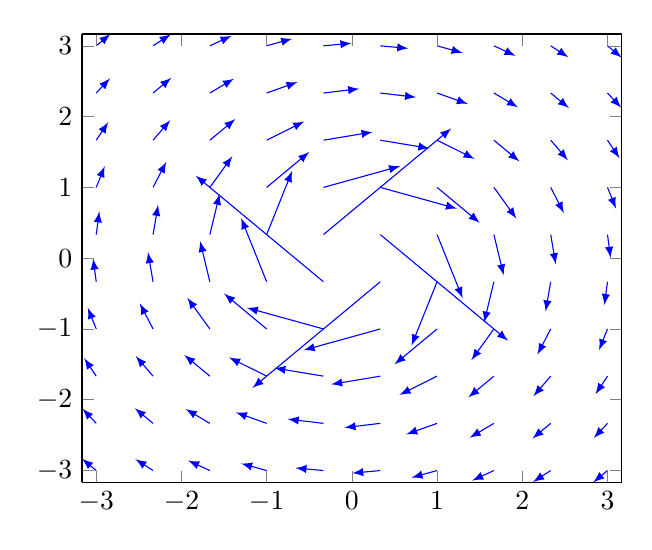
\begin{tikzpicture}
				\begin{axis}[%
					view     = {0}{90}, % for a view 'from above'
					domain   = -3:3,
					y domain = -3:3,
					xtick    = {-3,...,3},
					ytick    = {-3,...,3},
					]
					\addplot3[blue, quiver={u=y/(x*x+y*y), v=-x/(x*x+y*y), scale arrows=1}, samples=10, -latex] (x,y,0);
				\end{axis}
		\end{tikzpicture}}}
	\end{subcaptionbox}
	\caption{Vektorpfeile f\"{u}r $\va F_\eta^{(3)}$}
\end{figure}
	\begin{figure}[h!]
	\begin{subcaptionbox}{$\eta>-1$}
		{\resizebox{0.3\textwidth}{!}{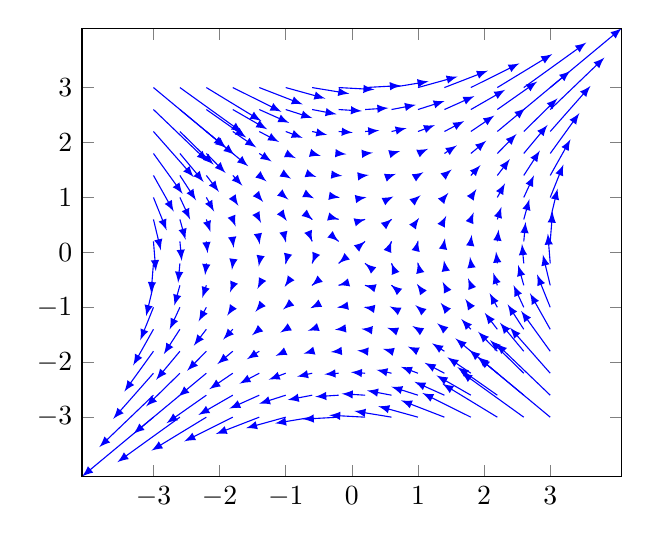
\begin{tikzpicture}
				\begin{axis}[%
					view     = {0}{90}, % for a view 'from above'
					domain   = -3:3,
					y domain = -3:3,
					xtick    = {-3,...,3},
					ytick    = {-3,...,3},
					]
					\addplot3[blue, quiver={u=(x*x+y*y)*y, v=(x*x+y*y)*x, scale arrows=0.02}, samples=16, -latex] (x,y,0);
				\end{axis}
		\end{tikzpicture}}}
		\begin{subcaptionbox}{$\eta=-1$}
			{\resizebox{0.3\textwidth}{!}{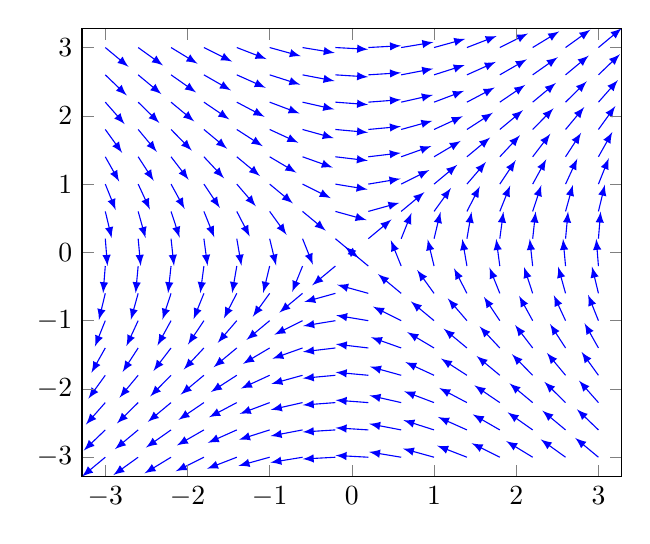
\begin{tikzpicture}
					\begin{axis}[%
						view     = {0}{90}, % for a view 'from above'
						domain   = -3:3,
						y domain = -3:3,
						xtick    = {-3,...,3},
						ytick    = {-3,...,3},
						]
						\addplot3[blue, quiver={u=y/(x*x+y*y)^(1/2), v=x/(x*x+y*y)^(1/2), scale arrows=0.4}, samples=16, -latex] (x,y,0);
					\end{axis}
			\end{tikzpicture}}}
		\end{subcaptionbox}
	\end{subcaptionbox}
	\begin{subcaptionbox}{$\eta<-1$}
		{\resizebox{0.3\textwidth}{!}{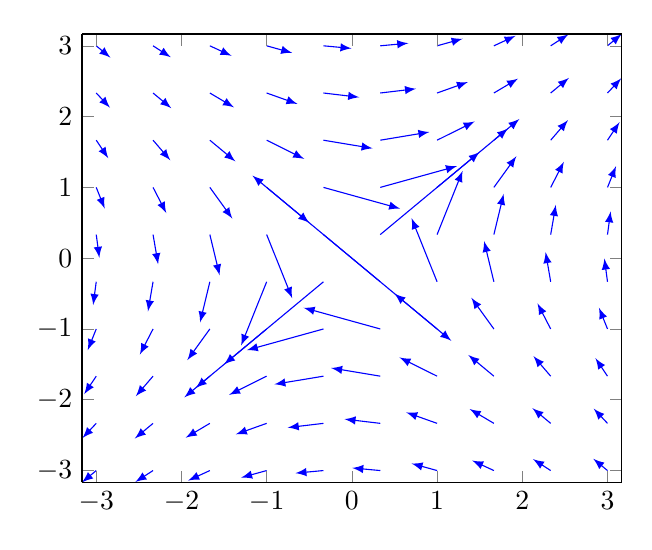
\begin{tikzpicture}
				\begin{axis}[%
					view     = {0}{90}, % for a view 'from above'
					domain   = -3:3,
					y domain = -3:3,
					xtick    = {-3,...,3},
					ytick    = {-3,...,3},
					]
					\addplot3[blue, quiver={u=y/(x*x+y*y), v=x/(x*x+y*y), scale arrows=1}, samples=10, -latex] (x,y,0);
				\end{axis}
		\end{tikzpicture}}}
	\end{subcaptionbox}
	\caption{Vektorpfeile f\"{u}r $\va F_\eta^{(4}$}
\end{figure}
\begin{enumerate}
	\item Maximalen Definitionsbereich (f\"{u}r alle $\va F_\eta^{(n)}$): Wenn $\eta\le -1, \R^3\backslash \{(0,0,0)\}$, sonst $\R^3$.
	\item maximale Bereiche, auf denen $\va F_\eta^{(n)}$ konservativ ist. $n=\dots$
	\begin{enumerate}[label=(\arabic*)]
		\item Falls $\eta=0,D_\eta^{(1)}$, sonst $z=0$
		\item Falls $\eta=0, D_\eta^{(2)}$, sonst $\varnothing$
		\item Falls $\eta=-2, D_\eta^{(3)}$, sonst $\varnothing$.
		\item Falls $\eta=0, D_\eta^{(4)}$, sonst $\varnothing$.
	\end{enumerate}
	\item Potentialfunktion, f\"{u}r $n=\dots$
	\begin{enumerate}[label=(\arabic*)]
		\item Auf $z=0$ Ebene:
		
		$\eta=-2$: $V=\frac 12\ln\left(x^2+y^2\right)$, sonst $V=\frac 1{\eta+2}r^{n+2}r^{n+2}$
	\end{enumerate}
\end{enumerate}
\end{proof}
\begin{Problem}
	Zwischen zwei Kreisringen mit Radius $R$, die bei $x = -x_0$ und $x = x_0$ zentriert in der $yz$-Ebene liegen, sei eine Seifenhaut gespannt (s. Skizze). Aufgrund der Oberflächenspannung wird sich die Seifenhaut so ausbilden, dass die entsprechende Oberfläche minimal ist.
	\begin{enumerate}
		\item Das gesamte Problem ist rotationssymmetrisch um die $x$-Achse. Zeigen Sie, dass die Fläche der Rotationsfigur um die $x$-Achse für die Funktion $y : [-x_0, x_0] \to \R$ zwischen den Kreisringen durch
			\[
				F(y)=\int_{-x_0}^{x_0} 2\pi y(x)\sqrt{1+y'(x)^2} \dd{x}	
	\] 
	mit $y'=\dv{y}{x}$ gegeben ist.

\item Benutzen Sie nun die in der Vorlesung kennengelernte Methode der Variationsrechnung, um die Minimalfläche zu finden, die von der Seifenhaut gebildet wird. Gesucht ist also die Funktion $y$, die $F (y)$ minimiert. (Hinweis: Zeigen Sie, dass die Euler-Lagrange-Gleichung für dieses Problem als
	\[
		\frac{1}{y'}\dv{x}\left( \frac{y}{\sqrt{1+y'^2} } \right) =0\] 
		geschrieben werden kann.)
	\end{enumerate}
	\begin{center}
	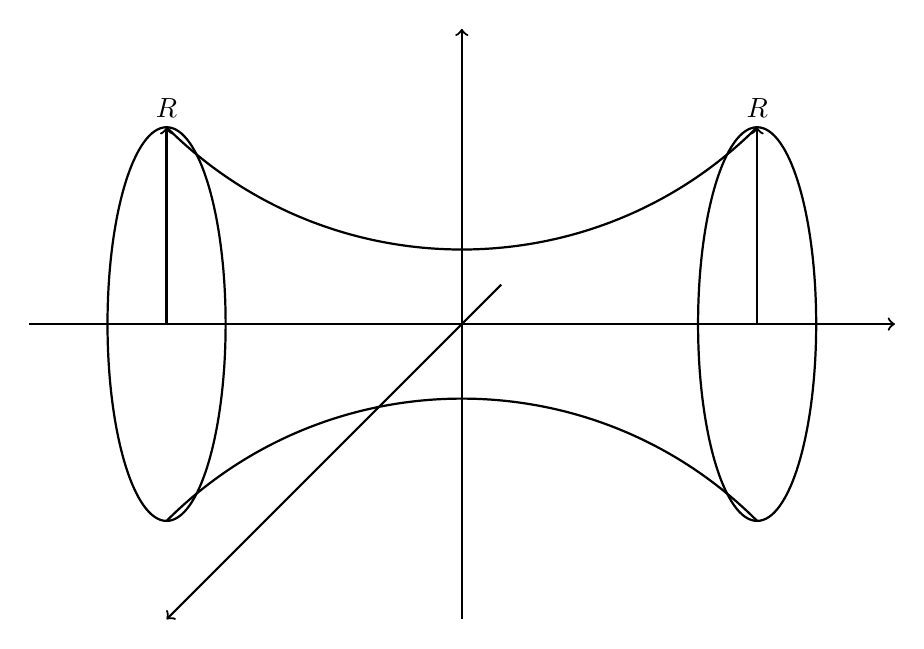
\begin{tikzpicture}[scale=2.5]
		\draw[thick, ->] (-2.2,0) -- (2.2,0);
		\draw[thick, ->] (0,-1.5) -- (0,1.5);
		\draw[thick] (-1.5,0) circle (0.3 and 1);
		\draw[thick] (1.5,0) circle (0.3 and 1);
		\draw[thick] (1.5,1) arc(-45:-135:{sqrt(4.5)});
		\draw[thick] (1.5,-1) arc(45:135:{sqrt(4.5)});
		\draw[thick, ->] (0.2,0.2) -- (-1.5,-1.5);
		\draw[thick,->] (-1.5,0) -- (-1.5,1);
		\draw (-1.5,1) node[anchor=south] {$R$};
		\draw[thick,->] (1.5,0) -- (1.5,1);
		\draw (1.5,1) node[anchor=south] {$R$};
	\end{tikzpicture}
\end{center}
\end{Problem}
